\documentclass[a4paper, 10pt, french]{article}
% Préambule; packages qui peuvent être utiles
   \RequirePackage[T1]{fontenc}        % Ce package pourrit les pdf...
   \RequirePackage{babel,indentfirst}  % Pour les césures correctes,
                                       % et pour indenter au début de chaque paragraphe
   \RequirePackage[utf8]{inputenc}   % Pour pouvoir utiliser directement les accents
                                     % et autres caractères français
   \RequirePackage{lmodern,tgpagella} % Police de caractères
   \textwidth 17cm \textheight 25cm \oddsidemargin -0.24cm % Définition taille de la page
   \evensidemargin -1.24cm \topskip 0cm \headheight -1.5cm % Définition des marges
   \RequirePackage{latexsym}                  % Symboles
   \RequirePackage{amsmath}                   % Symboles mathématiques
   \RequirePackage{tikz}   % Pour faire des schémas
   \RequirePackage{graphicx} % Pour inclure des images
   \RequirePackage{listings} % pour mettre des listings
% Fin Préambule; package qui peuvent être utiles

\title{Rapport de TP 4MMPOO : Simulation Orientée-Objet de systèmes multiagents }
\author{
MAHIEU Lucas (SL\_PHELMA) 
\\ DEVALON Hugues (SLE\_PHELMA) 
}

\begin{document}

\maketitle

%%%%%%%%%%%%%%%%%%%%%%%%%%%%%%%%%%%%%%%%%%%%%%%%%%%%%%%%%%%%%%%
\paragraph{\em Préambule}
{L’objectif de ce TP est de développer en Java des applications permettant de simuler de manière graphique des systèmes multiagents. Dans un premier temps, nous nous intéresserons à trois systèmes de type automate cellulaire : le jeu de la vie de Conway, un jeu de l’immigration, et le modèle de ségrégation de Schelling. Dans un second temps, nous nous intéresserons à la simulation d’un système de mouvement d’essaims auto-organisés : le modèle de Boids.
\\Nous vous proposons de lire la documentation disponible dans le repertoire doc\_gui\_jeux pour avoir les API de notre projet.
\\Nous présentons en figure~\ref{étiquette} page~\pageref{étiquette} la représentation UML des classes permettant la Simulation des l'automates cellulaires et des modélisations de {\em Boids}. Nous avons explicité les attributs privées des classes pour que vous compreniez mieux nos choix de conception et n'avons pas afficher certaine méthode par soucis de clarté.
}
\begin{figure}[h]
\hspace{-20mm} 
	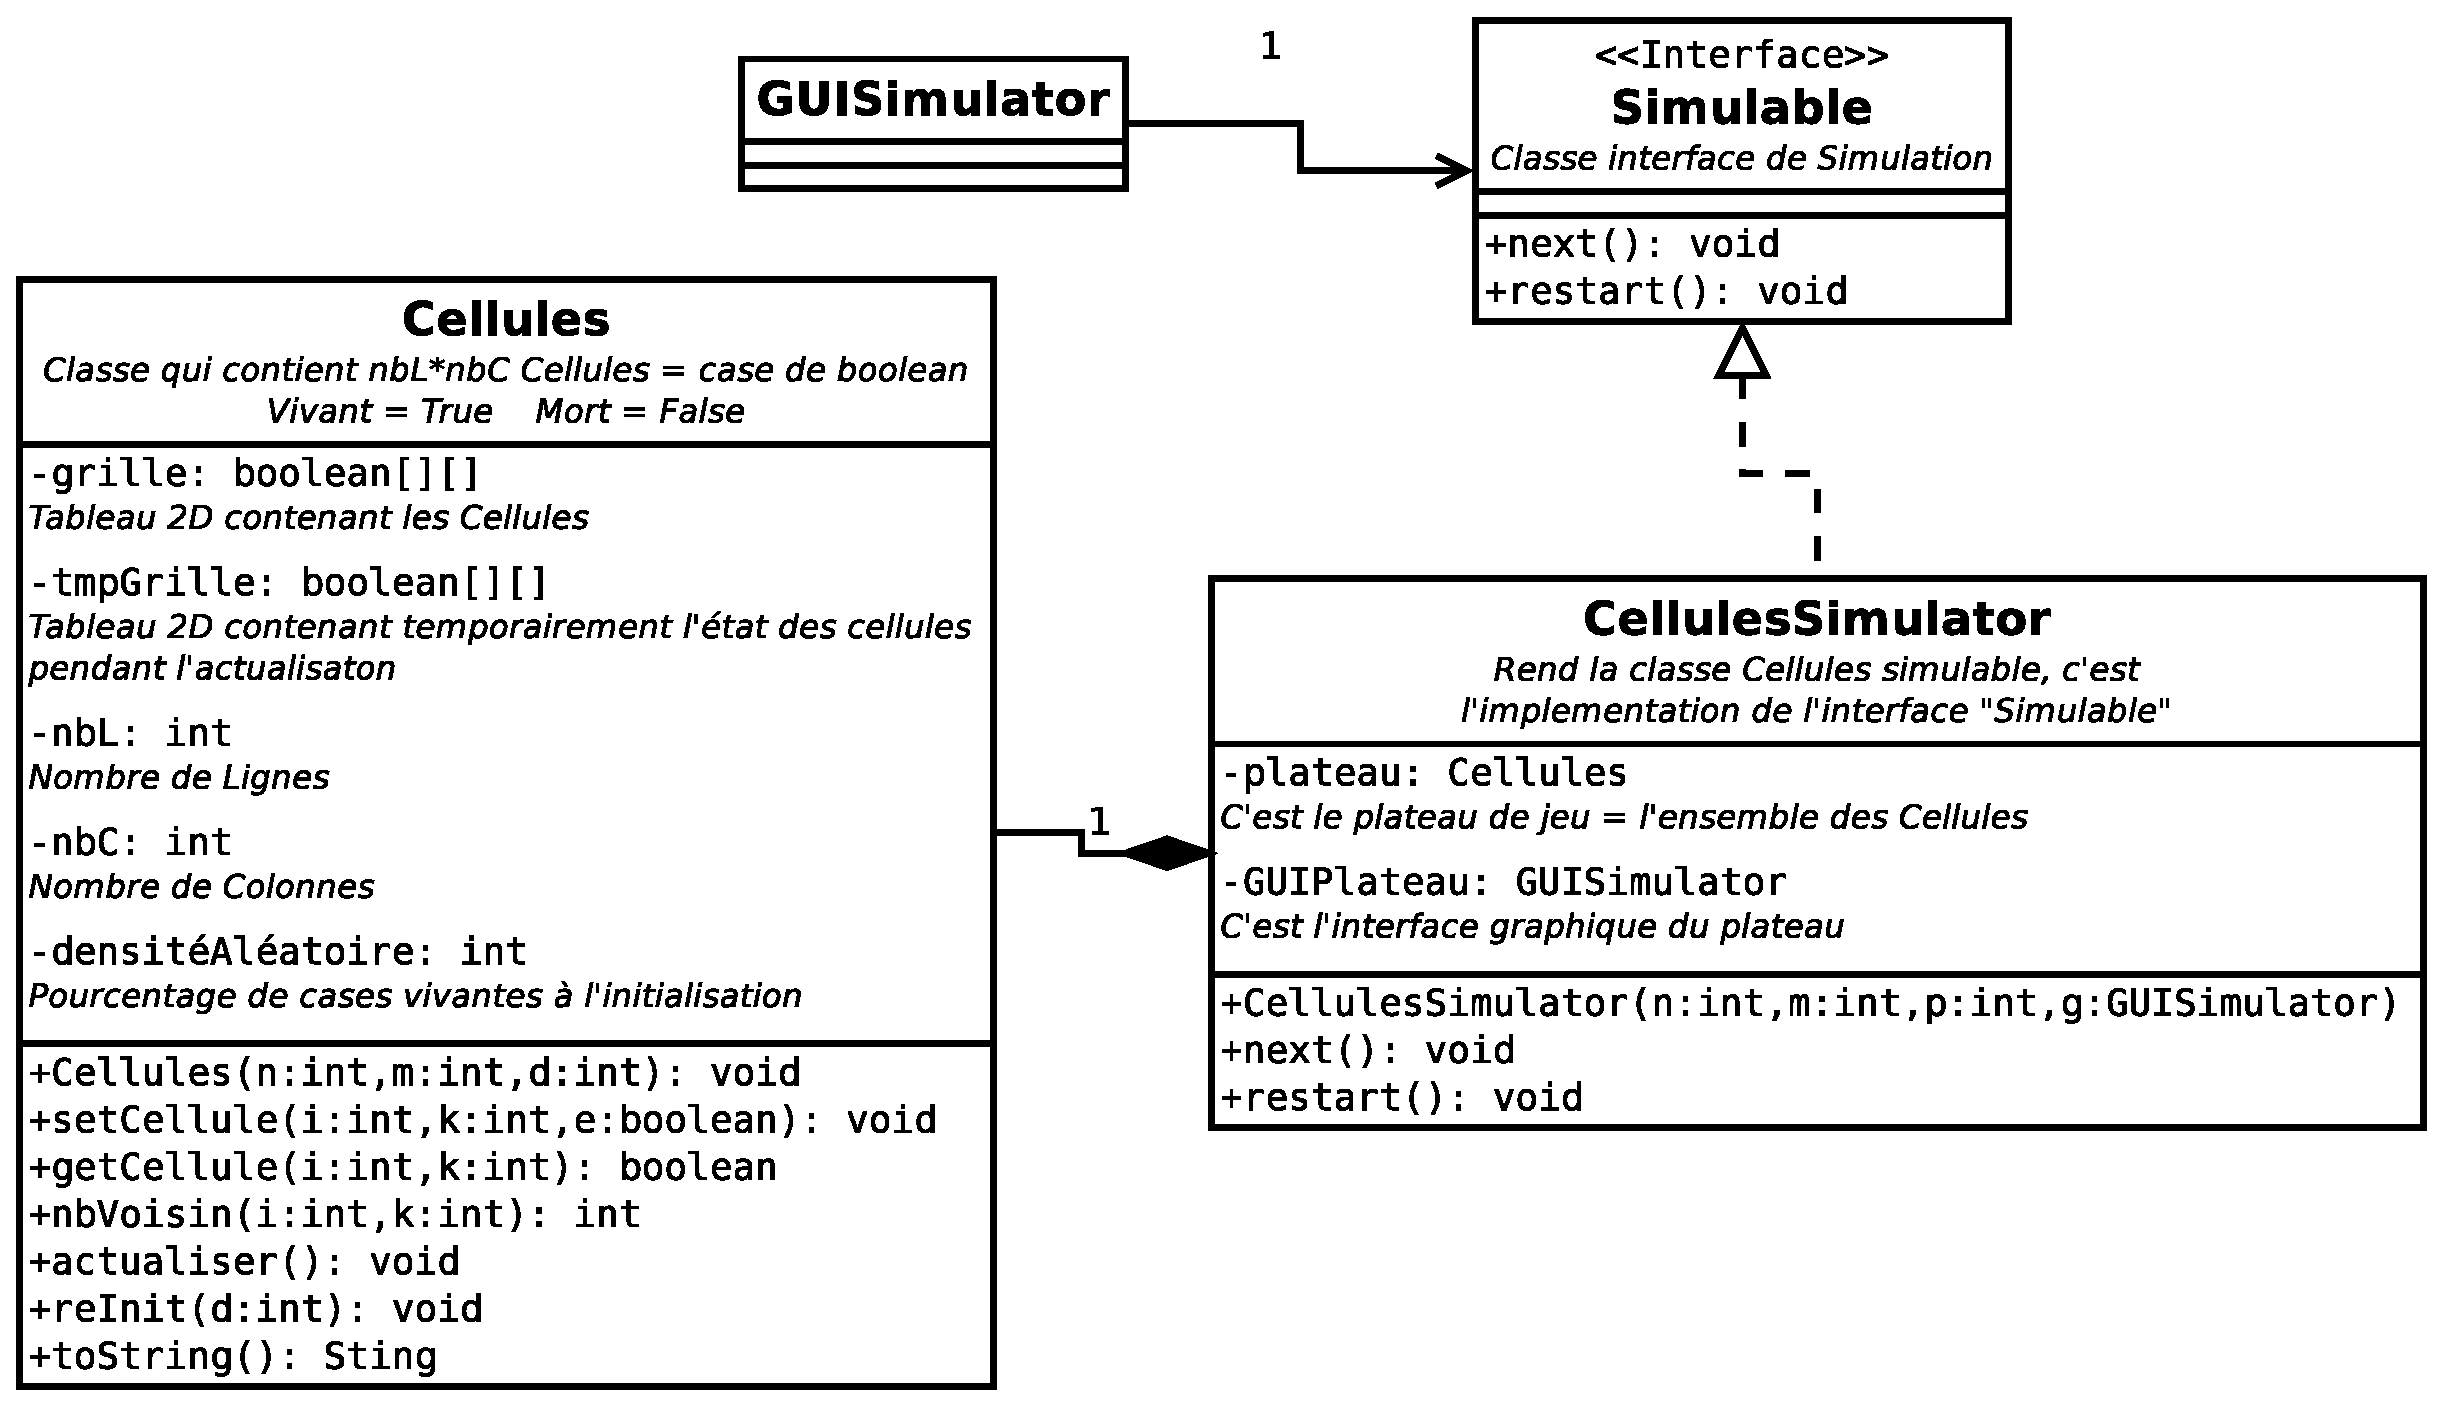
\includegraphics[scale=0.27]{UML_Cellules.eps}
	\caption{\label{étiquette} Diagramme des classes du jeu de la vie de Conway}
\end{figure}
%%%%%%%%%%%%%%%%%%%%%%%%%%%%%%%%%%%%%%%%%%%%%%%%%%%%%%%%%%%%%%%%
\section{Automates Cellulaires}
	\subsection{Jeu de la vie de Conway\,: }
		{Comme vous pouvez le constater, nous avons utilisé des classes assez 'génériques' pour qu'elles soient facilement réutilisables pour les autres jeux. De plus, on peut remarquer que notre conception est presque identique à celle proposée pour le jeux de balles. En effet, ici nous manipulons un tableau de {\em int} et non plus un tableau de {\em Point}. Ainsi pour l'adapter à d'autres jeux, il suffirait de modifier les correspondances entre les états et les couleurs et les règles d'actualisation.
\\ \indent Pour tester ces classes, nous avons utiliser deux classes de tests : l'une pour faire une simulation textuelle dans un premier tant, par la suite, quand la classe de calcule pour tester la simulation graphiquement.
		} 
%%%%%%%%%%%%%%%%%%%%%%%%%%%%%%%%%%
\subsection{Jeu de l'immigration\,:}
	{
Les seules différences avec le jeux de la vie sont 
	\begin{itemize}
		\item Qu'une cellule peut prendre un nombre {\em $n_e$} d'états et non plus seulement 2.
		\item Les règles de changement d'états.
	\end{itemize}
\indent Du fait que notre conception est générique, nous avons eu qu'à créer une nouvelle classe fille de {\em Cellules} qui implement une nouvelles méthode {\em actualiser()}{\em reInit()} propre au jeu de l'immigration. 
\\ \indent Nous avons fait le choix de créer une correspondance entre les {\em Entiers} qui représente l'état d'une cellule et une {\em Couleur} qui sera affichée dans sa simulation graphique. Pour ce faire nous avons utiliser une table de correspondance {\em Map<Integer, Color>}.
	}
%%%%%%%%%%%%%%%%%%%%%%%%%%%%%%%%%%
\subsection{Le modèle de Schelling\,:}
 	{ 
        \indent Pour cette partie, en plus d'avoir implémenté la nouvelle règle d'actualisation, nous avons utilisé une collection Java pour lister les habitations vacantes : {\em LinkedList}.
        De plus, nous avons considéré l'état -1 comme étant l'état d'une habitation vacante pour faciliter les calculs et faisant bien attention que ce nouvel état ne soit pas considéré comme une couleur lors du calcul des voisins.
        Lorsqu'une famille déménage, elle emménage dans une habitation vacante prise au hasard dans la liste.
        Lors de l'initialisation, toutes les habitations vacantes prévues sont créées dans l'ordre dans les premières cellules. Ce nombre de cellules vacantes dépend du facteur de ségrégation {\em k}, du nombre de lignes et du nombre de colonnes, selon la formule : $ \frac{lignes*colonnes}{5*(k+1)} $, trouvée empiriquement.
	} 

%%%%%%%%%%%%%%%%%%%%%%%%%%%%%%%%%%%%%%%%%%%%%%%%%%%%%%%%%%%%%%%
\section{Un modèle d'essaims\,: les {\em boids}}
  \subsection{Troupeaux de boids}
  {
  Pour implanter un simulateur de boids nous avons penser que le plus efficace serait de réutiliser ce que nous avions fait sur les balles. Ainsi nous avions qu'à étendre les propriétés des balles. En effet, un boids est une balles à laquelle on ajoute une information sur sa vitesse. Nous avons donc définit un tableau de {\em Vect2D} qui est ni plus ni moins qu'une extensions de la classe {\em Point} par soucis de clarté entre un point qui repère la position d'un boid et un vecteur qui repère sa vitesse.
  Un boid est donc repéré par sa position et sa vitesse. Ainsi pour que l'ensemble des boids se comporte en essaim, nous avons décidé d'appliquer les 3 règles de bases : la cohésion, l'alignement et la séparation.
  Chacune de ces règles est affectées d'un gain kC, kA, dS qui permettent de donner plus ou moins d'importance au groupe et ainsi de donner des comportements différents aux boids.
  }
%%%%%%%%%%%%%%%%%%%%%%%%%%%%%%%%%%%
    \subsubsection{Un gestionnaire à évènements discrets\,:} 
      {
      \indent Afin de gérer les événements dans {\em EventManager}, on utilise comme collection Java une {\em PriorityQueue} afin de classer les événements selon leur date d'execution de façon croissante. La classe {\em ComparateurDate} implémente cette relation de comparaison. La classe abstraire {\em Event} et ses sous-classes permettent de définir concrètement la nature des évènements.
      } 
%%%%%%%%%%%%%%%%%%%%%%%%%%%%%%%%%%%
    \subsubsection{Modification de votre simulateur\,: } 
      {
          \indent Grâce à la hierarchie des classes utilisés, il est facile d'utiliser les événements à la place de l'ancienne gestion. Il suffit alors de créer un sous-événement {\em BBEvent} pour les balles et les boids et {\em CellulesEvent} pour tous les types de jeu reposant sur les cellules.
      }
%%%%%%%%%%%%%%%%%%%%%%%%%%%%%%%%%%%
      \subsubsection{Simulation de plusieurs groupes de boids\,: } 
      {
          \indent Nous avons généralisé ce problème en proposant aussi de simuler plusieures groupes de balles, les boids étant des balles, cela ne posait pas de problème. Pour cela, il suffit simplement d'utiliser un tableau de balles partout où on les utilise, c'est à dire dans {\em BBEvent} et dans {\em BBSimulator} afin d'avoir un simulateur qui contient ces groupes de balles/de boids. Les événements sont alors communs : à la création du groupe on choisit leur délai d'attente entre deux execution, et leur événements s'ajoutent à la queue globale des événements.
      }

%%%%%%%%%%%%%%%%%%%%%%%%%%%%%%%%%%%%%%%%%%%%%%%%%%%%%%%%%%%%%%%
\section{Bilan}
{
Pour conclure ce projet, nous allons faire un bilan de notre travail: 
\begin{itemize}
		\item Ce projet nous a tout d'abord parus difficile à repartir entres les deux membres de notre équipe. Mais en s'organisant et en s'efforçant de diviser les tâches nous avons pu gagner beaucoup en efficacité.
		\item Du point de vu de l'organisation du code, nous avons utilisé Git qui nous a permis de gérer au mieux notre code.
		\item Le projet que l'on vous donne est selon nous abouti dans le sens où l'on a réussi à répondre à l'intégralité du sujet. Cependant avec un petit plus de temps nous aurions aimé ajouter quelques améliorations. 
		\begin{itemize}
			\item En effet, pour la simulation des boids, nous ne donnons pas d'angle de vision au boids, mais seulement une distance tout autour d'eux.
			\item Le deuxième point à améliorer serait la possibilité de faire interagir les différents groupes de boids entre eux. Option que nous n'avons pas eu le temps de créer. 
		\end{itemize}
		\item Pour le reste lancer notre jeu et laissez vous guider.
		\end{itemize}
}
%%%%%%%%%%%%%%%%%%%%%%%%%%%%%%%%%%%%%%%%%%%%%%%%%%%%%%%%%%%%%%%
\end{document}
%% Fin mise au format

